When considering the design space of mappings $M = A^K$ we usually consider no relationship between mappings. For two mappings we can say if they are identical or not, or perhaps with the methods of Chapter~\ref{chap:symmetries} if they are \emph{equivalent} or not. However, any further relationship we can't describe: can we say that two mappings are very similar, or very different? Can we quantify the \emph{distance} between two mappings? Intuitively, we can.

\begin{figure}[h]
	\centering
   \resizebox{0.55\textwidth}{!}{\begin{tikzpicture}
\draw (0,0) rectangle (5,5);
\draw (2.5,2.5) node {Placeholder};
\end{tikzpicture}
}
	\caption{An intuitive example of distance between mappings.}
	\label{fig:intuition_metric}
\end{figure}
Consider the example in \todo{write}.

We can formalize the intuition presented in the example from Figure~\ref{fig:intuition_metric}. Mathematically, a basic notion of distance is captured by the structure of a metric space. 
In this chapter we will thus show how to endow architecture graphs and mapping spaces with a metric space structure. While it allows for a simple and powerful mathematical definition, a metric space structure can be inefficient for calculations. To cope with this, we will also discuss low-distortion embeddings and show how we can find them for the metric spaces introduced.
Appendix~\ref{appendix:metric} reviews the basic notions of metric spaces, as well as more advanced concepts needed to introduce and find the more computationally efficient low-distortion embeddings.

\subsection{Architectures}

In the example illustrated in Figure~\ref{fig:intuition_metric} we saw intuitively how mappings can be more or less similar. This intuitive notion clearly depends on the underlying architecture. It is the hardware architecture that determines the cost of communicating data between processes. In order to endow the space of mappings with a metric space structure, we should first do so with the architecture.

The fundamental observation here is that in a multicore architecture, communication between different PEs takes different amounts of time. Consider, for example \todo{add example}.
There are multiple problems with using the communication time between PEs directly as a distance between PEs. Firstly, communication times depend on multiple factors: the latency and bandwith of the communication resources used, the amount of data being sent, the (software) communication protocol, clock synchronization between hardware resources like the PEs and buses, arbitration or other contention issues, etc.
Of course we can model these to various degrees. However, the distance between PEs needs to be a fixed number and not a function of all these factors. As an approximation, however, we can use the expected latency for a package of a standardized size (e.g. 8 bytes). As an expected value, this is a fixed number, but through its statistical nature it can include as much complexity in the model as required.

The second issue we run into when using communication times for defining a distance is that, by definition, the distance between a point and itself has to be $0$, but usually a PE has to communicate with itself using an $L1$ cache, scratchpad memory or similar, which has a small but non-zero latency. In this sense, the expected communication latency between cores is \textbf{not} a metric space distance, but it approximates one well. We propose thus to ignore this latency and set the distance to 0, to obtain the mathematical metric space structure. 

Finally, this metric space structure depends strongly on the unit used to measure latency (e.g. cycles, miliseconds, etc), as well as on the absolute speed of the communication subarchitecture.
Since the goal of exposing this structure is to leverage it for algorithmic decisions like finding good mappings, it is useful to have comparable distances between different architectures.
For this, we propose to norm the metric distance function such that the average distance between PEs is $1$.

Put together, these principles yield the following definition:
\begin{defn}[Architecture Metric Space]
Let $A = (P,E)$ be an architecture graph and $\operatorname{lat} : P -> P$ be the expected latency between PEs.
Then we set
\begin{align}
  d_A : P \times P, (p,q) \mapsto \left\{
      \begin{array}{rr}
        \operatorname{lat}(p,q), & \text{ if } p \neq q \\
        0, & \text{otherwise}
      \end{array} \right.
      \end{align}
\end{defn}
\begin{rem}
For an architecture graph $A = (P,E)$, the tuple $(P,d_A)$ is a metric space.
\begin{bew}
Obviously $d_A(p,p) = 0$ for all $p \in P$, by definition, and $d_A(p,q) > 0$ for $p \neq q$ since the expected latency between PEs is always greater than 0.
For $p,q,r \in P$ we have $d_A(p,q) + d_A(q,r) \geq d_A(p,r)$ since the expected latency of moving data from $p$ to $q$ and then to $r$ will always be at least as much as moving it from $p$ to $r$ directly.
\end{bew}
\end{rem}

\subsubsection{Application distances}

\subsection{Mappings}
\begin{figure}[h]
	\centering
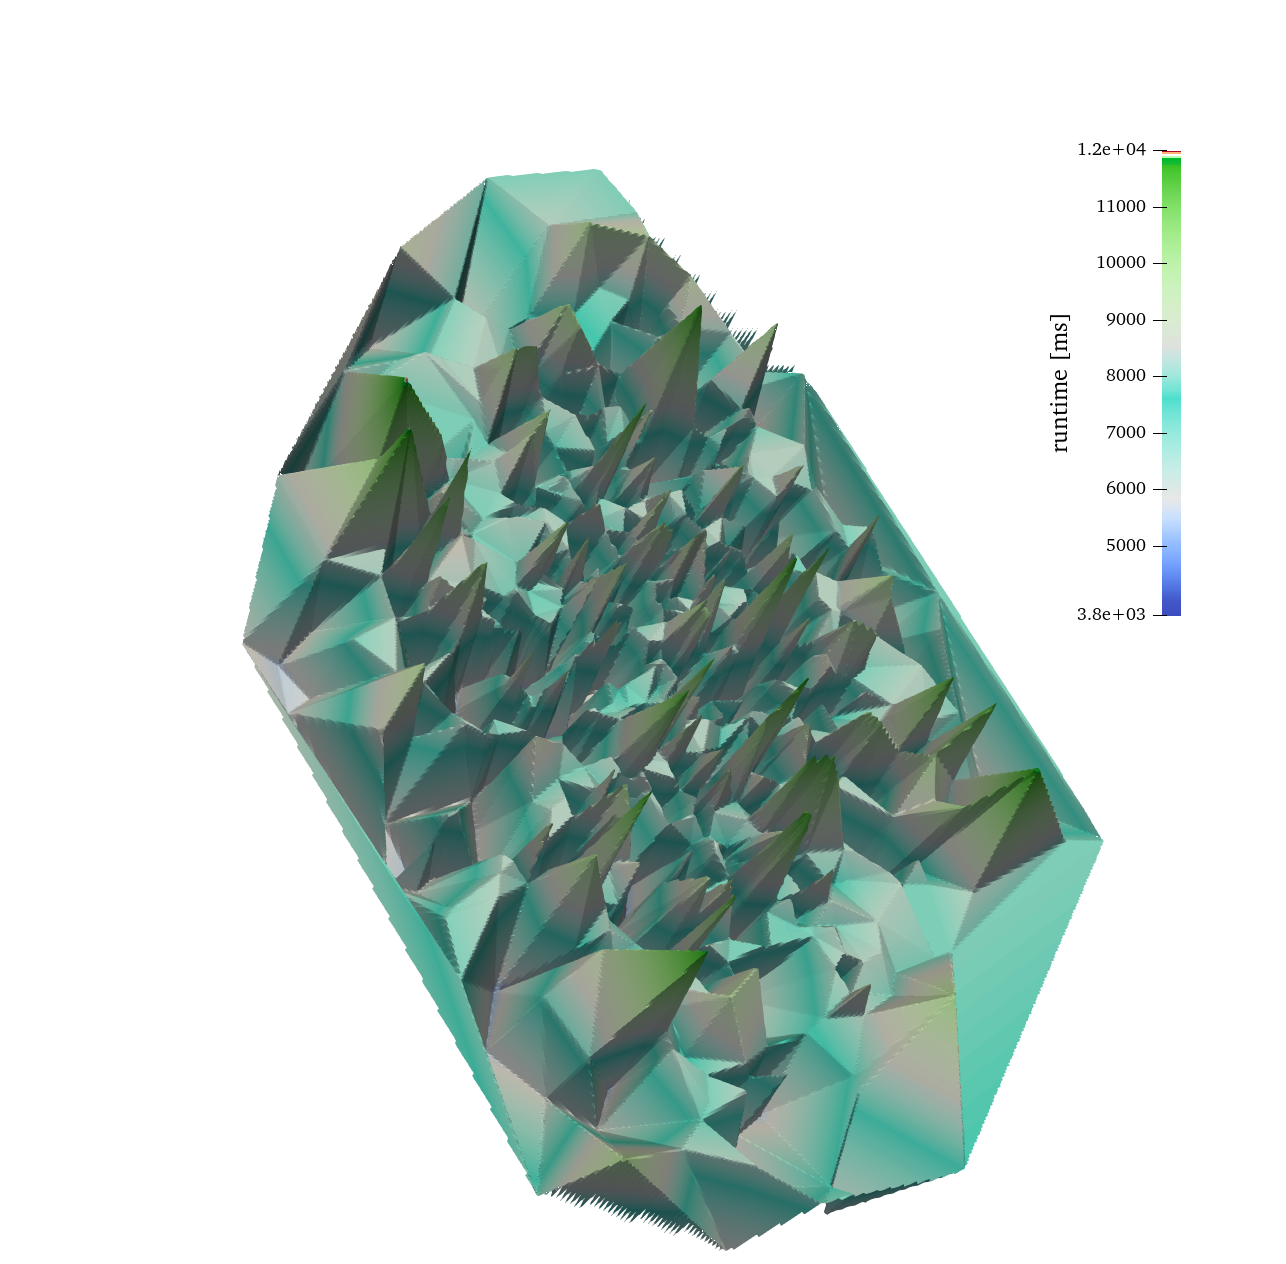
\includegraphics[width=\textwidth]{figures/coolidge-af-space3.png}
	\caption{A visualization of a random projection of the mapping space}
	\label{fig:mapping_space}
\end{figure}

\subsection{Low-distortion Embeddings}

\begin{figure}[h]
	\centering
   \resizebox{0.95\textwidth}{!}{\inputTikz{metric_spaces_comparison_exynos.tex}}
	\caption{Comparison of multiple distance metrics on the Odroid XU4 platform.}
	\label{fig:metric_comparison}
\end{figure}

\begin{figure}[h]
	\centering
   \resizebox{0.95\textwidth}{!}{\inputTikz{metric_spaces_comparison_max_exynos.tex}}
	\caption{Comparison of multiple distance metrics as predictors of the \emph{maximal} run-time difference on the Odroid XU4 platform.}
	\label{fig:metric_comparison_max}
\end{figure}
\begin{figure}[h]
	\centering
   \resizebox{0.95\textwidth}{!}{\inputTikz{metric_spaces_comparison_coolidge.tex}}
	\caption{Comparison of multiple distance metrics on the MPPA3 Coolidge platform.}
	\label{fig:metric_comparison}
\end{figure}

\begin{figure}[h]
	\centering
   \resizebox{0.95\textwidth}{!}{\inputTikz{metric_spaces_comparison_max_coolidge.tex}}
	\caption{Comparison of multiple distance metrics as predictors of the \emph{maximal} run-time difference on the MPPA3 Coolidge platform.}
	\label{fig:metric_comparison_max}
\end{figure}


\begin{figure}[h]
	\centering
   \resizebox{0.75\textwidth}{!}{\input{generated/metrics_regression_rsq.tex}}
	\caption{Comparison of the predictive power of multiple distance metrics.}
	\label{fig:metric_regression}
\end{figure}
